%%
%% Guardian Chip – LAYR Open Chip Challenge 25/26
%% Academic Report
%%
%% Build: pdflatex main.tex && bibtex main && pdflatex main.tex && pdflatex main.tex
%%
\documentclass[manuscript,screen,nonacm]{acmart}

% ---------------------------------------------------------------
% Packages
% ---------------------------------------------------------------
\usepackage{microtype}
\usepackage{booktabs}
\usepackage{listings}
\usepackage{xcolor}
\usepackage{subcaption}
\usepackage{cleveref}
\usepackage{rotating}    % sidewaysfigure for wide diagrams
\usepackage{graphicx}    % ensure \includegraphics options work
\usepackage{float}       % [H] placement specifier

% Code listing style
\lstdefinestyle{verilog}{
  language        = Verilog,
  basicstyle      = \ttfamily\small,
  keywordstyle    = \color{blue}\bfseries,
  commentstyle    = \color{gray}\itshape,
  stringstyle     = \color{orange},
  numbers         = left,
  numberstyle     = \tiny\color{gray},
  frame           = single,
  breaklines      = true,
  tabsize         = 2,
  showstringspaces= false
}

% ---------------------------------------------------------------
% Document metadata
% ---------------------------------------------------------------
\title{Guardian Chip: A Compact NFC Access-Control ASIC\\
       with Mutual AES-128 Authentication}

\author{Philipp Seelos}
\affiliation{%
  \institution{Hochschule RheinMain}
  \country{Germany}
}
\email{philipp.seelos@student.hs-rm.de}

\thanks{This work was carried out as part of the course
\emph{Advanced IC Design} at Hochschule RheinMain,
supervised by Prof.\,Dr.\ Steffen Reith.}

\begin{abstract}
This report documents the design and implementation of the \emph{Guardian Chip},
a custom application-specific integrated circuit (ASIC) developed for the
LAYR Open Chip Challenge~2025/26~\cite{ocdc_layr}.
The chip implements a hardware door-lock controller that authenticates
contactless smart cards using the LAYR Level~1 Authenticated Identification
Protocol, a symmetric challenge-response protocol based on AES-128.

The design is described in Verilog/SystemVerilog and targets the
IHP~SG13G2 130\,nm BiCMOS open-source process~\cite{ihpsg13g2},
to be fabricated as a QFN-24 package via the LibreLane open-source ASIC
flow~\cite{librelane}.
The chip communicates with an NXP~MFRC522 NFC reader~\cite{mfrc522}
and a Microchip AT25010B SPI~EEPROM~\cite{at25010b} over a shared
4\,MHz SPI bus.
The authentication logic performs a mutual challenge-response handshake,
derives an ephemeral session key, decrypts the card identity,
and checks the result against a six-entry whitelist stored in non-volatile
memory.
AES-128 is realised as a compact iterative engine that processes one
round per clock cycle and uses a compact composite-field
S-box~\cite{canright2005,canright_github} to minimise silicon area.
The mathematical foundation for this S-box was established by
Canright~\cite{canright2005}; the Verilog implementation used in this
work was published by GitHub user \emph{coorus}~\cite{canright_github}.
Beyond the standard LAYR~Level~1 protocol, a key-rollover mechanism
was designed and implemented that allows the pre-shared key to be
updated over the air as part of a successfully authenticated
transaction.
To allow seamless software-level testing without physical JavaCards,
a companion Android Host Card Emulation (HCE) application that fully
implements the card side of the protocol was also developed.
\end{abstract}

\keywords{ASIC, NFC, AES-128, challenge-response authentication,
          SPI, EEPROM, open-source PDK, access control, LAYR}

\begin{document}
\maketitle

% ===============================================================
\section{Introduction}
\label{sec:intro}
% ===============================================================

Physical access control is a fundamental problem in security engineering.
Traditional keycard systems either store the permitted identifiers in
plaintext and send them unencrypted over the wireless link—making replay
attacks trivial~\cite{hancke2005relay}—or rely on proprietary, poorly
documented protocols whose security is hard to reason about.

The LAYR Open Chip Challenge~\cite{ocdc_layr} poses exactly this problem:
design a microchip that controls a 12\,V door lock, reads a contactless
smart card via ISO~14443-A/4~\cite{iso14443-3,iso14443-4}, and decides
whether to grant access.
The challenge defines four security levels; this work targets
\emph{Level~1}, which mandates the \emph{LAYR Authenticated Identification
Protocol}: a symmetric, AES-based mutual challenge-response scheme that
provides both card-to-terminal and terminal-to-card authentication and
establishes a fresh ephemeral session key for every transaction.

Beyond the mandatory protocol requirements, a key-rollover mechanism
was developed as an additional security feature that enables the
pre-shared key to be updated over the air as part of an authenticated
transaction, without requiring physical EEPROM access.

Rather than targeting an FPGA prototype only, the goal is to produce a
tape-out-ready ASIC.
The chip is designed with the IHP~SG13G2 130\,nm open-source PDK,
synthesised and placed-and-routed with the LibreLane flow,
and packaged in a QFN-24 footprint as specified by the challenge.

The remainder of this report is organised as follows.
Section~\ref{sec:related} reviews related work on compact hardware AES
and NFC security.
Section~\ref{sec:arch} describes the system architecture.
Section~\ref{sec:security} analyses the security of the implemented
protocol.
Section~\ref{sec:impl} details each RTL module.
Section~\ref{sec:simulator} presents the Android companion application.
Section~\ref{sec:physical} covers the physical design.
Section~\ref{sec:process} outlines the development process.
% TODO: fill in verification section once test results are finalised
Section~\ref{sec:verification} describes the verification strategy.
Section~\ref{sec:discussion} discusses limitations and future work,
and Section~\ref{sec:conclusion} concludes the report.

% ===============================================================
\section{Related Work}
\label{sec:related}
% ===============================================================

\paragraph{Compact hardware AES.}
Implementing AES in hardware with a small footprint is well studied.
Satoh~et~al.~\cite{satoh2001} showed that a composite-field
representation of GF($2^8$) over GF($2^4$) allows the S-box to be
realised with significantly fewer gates than a lookup-table approach.
Canright~\cite{canright2005} refined this into an extremely compact
algebraic construction.
A Verilog implementation of this design was published by GitHub
user \emph{coorus}~\cite{canright_github} and is adopted in this work.
Feldhofer~et~al.~\cite{feldhofer2004rfid} demonstrated that AES is
practical for RFID devices with strong resource constraints.

\paragraph{NFC and RFID security.}
Hancke and Kuhn~\cite{hancke2005relay} formalised relay attacks against
contactless cards, motivating the need for challenge-response schemes
that cannot be relayed without increasing round-trip latency.
The LAYR protocol addresses this at the application layer.
Host Card Emulation (HCE) on Android, introduced in Android~4.4,
enables a smartphone to emulate an ISO~14443-4 card without requiring
a hardware Secure Element, which is exploited for the companion
simulator in Section~\ref{sec:simulator}.

\paragraph{Challenge-response authentication.}
The protocol structure—each party encrypts a nonce from the other party
and returns the result—is a well-known symmetric authentication
pattern~\cite{dolev1983protocol}.
The specific instantiation used by LAYR derives a fresh ephemeral key
from the exchanged nonces, similar in spirit to the key derivation
used in EMV contactless~\cite{emvco2014}.

% ===============================================================
\section{System Architecture}
\label{sec:arch}
% ===============================================================

\subsection{Overview}
\label{sec:arch:overview}

\Cref{fig:arch} shows the top-level architecture.
The chip integrates five main RTL subsystems around a shared SPI bus:

\begin{enumerate}
  \item \textbf{SPI Master} – a byte-oriented SPI~Mode~0 master clocked
        at 4\,MHz, shared by both the NFC reader and the EEPROM.
  \item \textbf{NFC Interface} (\texttt{mfrc522\_apdu\_interface}) –
        drives the MFRC522 reader, performs ISO~14443-A card detection,
        brings up an ISO~14443-4 link (RATS / ATS exchange), and
        provides a byte-stream APDU interface to the LAYR authentication core.
  \item \textbf{LAYR Core} (\texttt{layr\_core}) – implements the
        complete state machine for the LAYR Level~1 protocol,
        including a key-rollover extension designed beyond the
        standard LAYR specification.
  \item \textbf{AES Core} (\texttt{aes\_core} / \texttt{aes\_iterative})
        – a compact iterative AES-128 engine used for all encryption
        and decryption operations in the authentication core.
  \item \textbf{EEPROM Interface} (\texttt{at25010\_interface}) –
        reads the pre-shared key, the nonce counter, and the ID
        whitelist from the AT25010B on power-up, and persists updated
        values when required.
\end{enumerate}

\begin{figure}[ht]
  \centering
  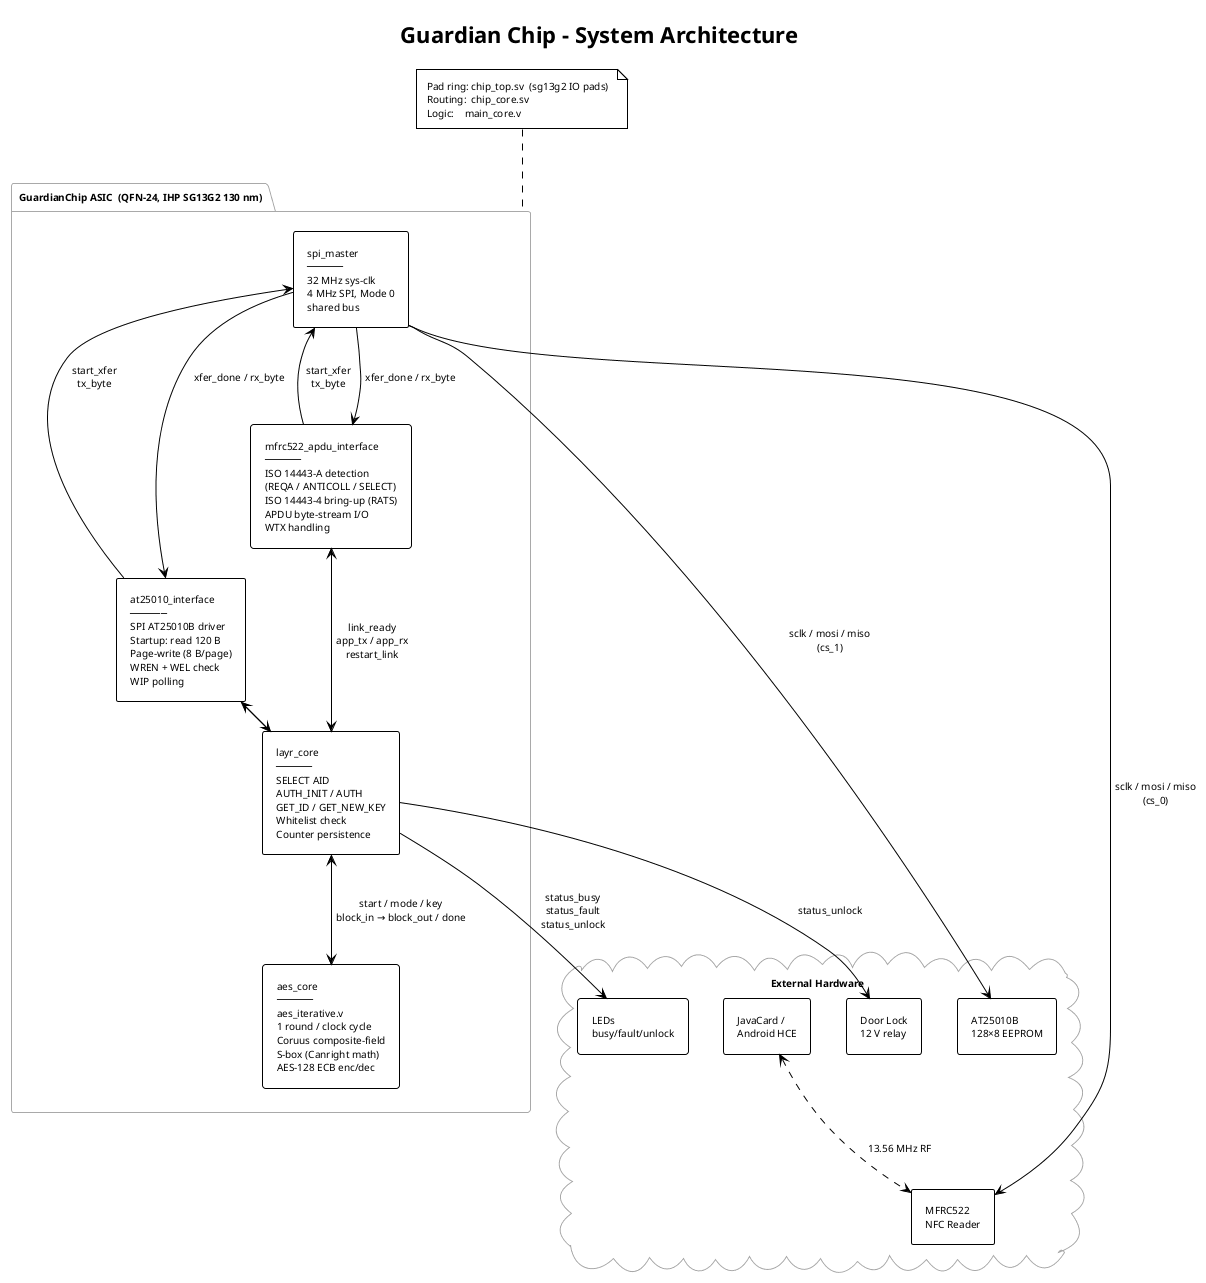
\includegraphics[width=\linewidth, height=0.88\textheight, keepaspectratio]{figures/system_arch.png}
  \caption{System architecture of the Guardian Chip.
           Arrows denote the direction of primary data flow.
           The SPI bus (sclk, mosi, miso) is shared; CS lines select
           the active peripheral.}
  \label{fig:arch}
\end{figure}

\subsection{Pin Interface and Packaging}
\label{sec:arch:pins}

The chip is packaged in a QFN-24 footprint as required by the LAYR
challenge specification~\cite{ocdc_layr}.
\Cref{tab:pins} lists the externally used pins.
The remaining pins carry power and ground rails.
Five bidirectional user-IO pads are present in the pad ring but are
currently held as inputs (unused) and reserved for future use.

\begin{table}[ht]
  \caption{Externally used signal pins (QFN-24).}
  \label{tab:pins}
  \centering
  \begin{tabular}{llll}
    \toprule
    Pin & Name & Direction & Function \\
    \midrule
    1  & \texttt{rst}          & Input  & Active-high synchronous reset \\
    2  & \texttt{sys\_clk}     & Input  & System clock (32\,MHz) \\
    13 & \texttt{cs\_1}        & Output & AT25010B SPI chip-select \\
    14 & \texttt{cs\_0}        & Output & MFRC522 SPI chip-select \\
    15 & \texttt{spi\_miso}    & Input  & SPI data from peripheral \\
    16 & \texttt{spi\_mosi}    & Output & SPI data to peripheral \\
    17 & \texttt{spi\_sclk}    & Output & SPI clock \\
    20 & \texttt{status\_unlock} & Output & Green LED / relay unlock \\
    21 & \texttt{status\_fault}  & Output & Red LED (authentication error) \\
    22 & \texttt{status\_busy}   & Output & Yellow LED (transaction in progress) \\
    \bottomrule
  \end{tabular}
\end{table}

\subsection{Module Hierarchy}
\label{sec:arch:hier}

\begin{description}
  \item[\texttt{chip\_top.sv}]
    Instantiates all IHP~SG13G2 pad cells: power pads (\texttt{IOPadVdd},
    \texttt{IOPadVss}, \texttt{IOPadIOVdd}, \texttt{IOPadIOVss}),
    unidirectional input/output pads, and bidirectional tri-state pads.
    Provides the polarity inversion for the active-low internal reset
    from the active-high external pin.

  \item[\texttt{chip\_core.sv}]
    Routes signals between pad cells and the main logic core.
    Holds the pin-to-signal mapping table as comments for
    traceability.

  \item[\texttt{main\_core.v}]
    Integration level: instantiates the SPI master, the NFC interface,
    the EEPROM interface, and the LAYR core.
    Multiplexes the SPI master between the two consumers: the EEPROM
    interface has priority during its power-on read sequence; after
    that, the NFC interface takes control.
    The NFC interface is kept in reset (\texttt{rst | eeprom\_busy})
    while the EEPROM is loading, ensuring that NFC activity cannot
    interfere with key retrieval.
\end{description}

% ===============================================================
\section{Security Analysis and Protocol Design}
\label{sec:security}
% ===============================================================

\subsection{Threat Model}
\label{sec:security:threat}

We consider an adversary with the following capabilities:

\begin{itemize}
  \item \emph{Passive eavesdropping.} The attacker can observe all
        wireless messages between card and reader.
  \item \emph{Active relay.} The attacker can inject, modify, or replay
        recorded messages within the same session or across sessions
        (replay attack).
\end{itemize}

We explicitly \emph{exclude} the following threats from the scope of
this level:
Side-channel attacks on the AES core (Level~2 requirement),
fault-injection attacks (Level~3 requirement),
and compromise of the EEPROM key storage (explicitly excluded by the
challenge specification).

\subsection{LAYR Level~1 Protocol}
\label{sec:security:protocol}

The LAYR Authenticated Identification Protocol~\cite{layr_javacard}
is a symmetric mutual challenge-response scheme executed over
ISO~14443-4 APDU commands.
Both parties share a 128-bit pre-shared key~$k_\text{psk}$.

\paragraph{Protocol flow.}
The chip (terminal) initiates the exchange after detecting a card:

\begin{enumerate}
  \item \textbf{SELECT AID.} The terminal selects the LAYR applet
        by its application identifier \texttt{F000000CDC01}.

  \item \textbf{AUTH\_INIT (INS=0x10).}
        The card draws a random 8-byte nonce~$r_C$, computes
        $c_C = \text{AES}_{k_\text{psk}}(r_C \,\|\, 0^{64})$, and
        returns $c_C$.
        The terminal decrypts $c_C$ and recovers $r_C$.
        This proves (to the terminal) that the card knows $k_\text{psk}$.

  \item \textbf{AUTH (INS=0x11).}
        The terminal generates its own 8-byte nonce~$r_T$ using a
        counter-based CTR construction
        ($r_T = \text{AES}_{k_\text{psk}}(0^{64}\,\|\,\mathit{ctr})_{\text{lo}64}$),
        increments the counter, and computes
        $c_T = \text{AES}_{k_\text{psk}}(r_T \,\|\, r_C)$.
        The ephemeral session key is formed as
        $k_\text{eph} = r_C \,\|\, r_T$.
        The terminal sends $c_T$ to the card.

  \item The card decrypts $c_T$ to recover $r_T$ and $r_C$.
        It verifies that the received $r_C$ matches the value it
        generated in step~2, proving that the terminal knows
        $k_\text{psk}$.
        The card also forms $k_\text{eph} = r_C \,\|\, r_T$.
        It responds with
        \[\text{AES}_{k_\text{eph}}(\texttt{"AUTH\_SUCCESS"} \| 0^{32}).\]

  \item \textbf{GET\_ID (INS=0x12).}
        The terminal sends a GET\_ID command.
        The card responds with $\text{AES}_{k_\text{eph}}(\mathit{id})$,
        where $\mathit{id}$ is the 128-bit card identity.
        The status word \texttt{0x9001} instead of \texttt{0x9000}
        indicates that the card has a new key ready for rollover.

  \item The terminal decrypts the identity and checks it against
        the six-slot whitelist loaded from the EEPROM.
        If the identity is in the list, the \texttt{status\_unlock}
        output is asserted for 3\,seconds.
\end{enumerate}

\paragraph{Security properties.}
Freshness of $r_C$ is guaranteed by the card's random number generator.
Freshness of $r_T$ is guaranteed by the monotonic counter stored in
non-volatile EEPROM memory: even after a power cycle the counter never
repeats, so the terminal nonce is never reused.
The ephemeral key $k_\text{eph}$ is session-unique; intercepting one
session does not help an attacker in a future session.
The AUTH step in direction terminal~→~card also serves as a proof of
key knowledge, providing mutual authentication.

\paragraph{Resistance to replay.}
Each session uses a fresh $r_C$ (random) and a fresh $r_T$
(counter-derived).
Replaying a captured $c_T$ from a previous session will fail at the
card's $r_C$ verification because $r_C$ will differ.
Replaying a captured session entirely is prevented because
$r_C$ is a fresh random value chosen by the card.

\subsection{Key Rollover}
\label{sec:security:rollover}

To support periodic key rotation without manual EEPROM reprogramming,
the protocol includes an optional key-rollover extension.
When the card returns \texttt{SW=0x9001} in step~5, the terminal sends
an additional \textbf{GET\_NEW\_KEY (INS=0x21)} command.
The card responds with $\text{AES}_{k_\text{eph}}(k_\text{new})$,
the new key encrypted under the established ephemeral key.
The terminal decrypts $k_\text{new}$, writes it to the EEPROM
(replacing $k_\text{psk}$), and only then asserts the unlock signal.

This mechanism ensures that a key update only takes effect after a
successfully authenticated transaction, preventing denial-of-service
through rogue key injection (which would require knowing $k_\text{psk}$
to forge $k_\text{eph}$).

% ===============================================================
\section{RTL Implementation}
\label{sec:impl}
% ===============================================================

\subsection{Shared SPI Master (\texttt{spi\_master.v})}
\label{sec:impl:spi}

A single SPI master instance is shared between the MFRC522 and the
AT25010B by a simple priority multiplexer in \texttt{main\_core.v}:
the EEPROM interface holds priority during its power-on read;
afterwards the NFC interface drives the bus.
The master operates in SPI Mode~0 (CPOL=0, CPHA=0), transmits MSB
first, and exposes a one-byte handshake interface (\texttt{start\_xfer},
\texttt{tx\_byte}, \texttt{xfer\_done}, \texttt{rx\_byte}).
The SPI clock is derived from the 32\,MHz system clock by a
counter-based divider, configurable at synthesis time via the
\texttt{CLK\_HZ} and \texttt{SPI\_HZ} parameters.
The default configuration produces a 4\,MHz SPI clock (8-cycle period).

\subsection{NFC Front-End Interface (\texttt{mfrc522\_apdu\_interface.v})}
\label{sec:impl:nfc}

This module is responsible for all communication with the MFRC522
NFC reader chip and the underlying card.
It operates in four main phases, shown in \cref{fig:nfc_state}:

\paragraph{Phase~0 – Reset and initialization.}
To get the reader into a state where it can detect cards,
the module issues a \texttt{SoftReset} to the MFRC522, writes the operating
registers (modulation, antenna, gain, timer), and reads back the \texttt{Version}
register to confirm the chip is present before advancing to card detection.


\paragraph{Phase~1 – ISO~14443-A card detection.}
The module periodically sends a REQA command (\texttt{0x26})
through the MFRC522's Transceive function.
On receiving an ATQA response it executes the anti-collision loop
(single-cascade UID) and the SELECT command to bring the card into
ACTIVE state.

\paragraph{Phase~2 – ISO~14443-4 link bring-up.}
After a successful SELECT, the module sends a RATS (Request for
Answer To Select) frame with parameters suitable for a JavaCard
(FSDI=8, DID=0).
The module receives the ATS (Answer To Select), enables ISO~14443-4
CRC mode on both transmit and receive paths of the MFRC522,
re-configures the MFRC522 timer registers (\texttt{TMode} and
\texttt{TPrescaler}) explicitly for the APDU phase,
and then waits for the mandatory Start-up Frame Guard Time (SFGT)
of approximately 10\,ms before asserting \texttt{link\_ready}.
The SFGT wait states (\texttt{APDU\_CFG2\_TMODE},
\texttt{APDU\_CFG2\_TPRESCALER}, \texttt{APDU\_ATS\_SFGT\_WAIT})
are explicitly excluded from the \texttt{link\_ready} condition
so that the LAYR core cannot begin an APDU transaction before the
card is ready to receive the first frame.

\paragraph{Phase~3 - APDU exchange.}
Once \texttt{link\_ready} is asserted, the module transparently
forwards APDU bytes between the application layer (\texttt{app\_tx}/
\texttt{app\_rx}) and the card, framing them in ISO~14443-4 I-blocks.
It handles block numbering, WTX (waiting-time-extension) acknowledge
frames, and error detection via the MFRC522's error register.
WTX frames require a minimum of two bytes (PCB + WTXM), while
normal I-blocks require at least three (PCB + SW1 + SW2); the
receive length check was corrected accordingly to avoid rejecting
valid WTX frames.
When a timer interrupt fires without a simultaneously pending
error bit (TimerIRq alone), the module performs a soft restart
of the card-detection loop rather than signalling a hard fault,
which enables graceful recovery when the card does not respond to
RATS or to an individual APDU.
The \texttt{block\_num} counter is explicitly reset to zero on
every soft or hard restart to avoid I-block sequence-number
mismatch on the next transaction.
The module asserts \texttt{hard\_fault} and restarts from the
hard-reset state only on unrecoverable (CRC or framing) errors.

% Figure~\ref{fig:nfc_state} is placed at the end of the document (wide sideways figure).

\subsection{AES Engine (\texttt{aes\_core.v} / \texttt{aes\_iterative.v})}
\label{sec:impl:aes}

The AES engine is a compact iterative design that executes one
AES-128 round per clock cycle.
It supports both encryption and decryption, selected by a \texttt{mode}
signal.
The key schedule is also computed iteratively (one round key per cycle)
to avoid a long combinatorial path.

\paragraph{S-box implementation.}
To minimise area, the S-box uses the composite-field construction
whose mathematical theory was developed by Canright~\cite{canright2005}.
The concrete Verilog implementation is taken from the open-source
repository published by GitHub user \emph{coorus}~\cite{canright_github}.
This S-box operates over GF($2^4$) / GF($2^2$) tower-field arithmetic
and avoids all ROM-based lookup tables, resulting in significantly
fewer standard cells than a conventional LUT approach.

\paragraph{Timing.}
A complete AES-128 encryption or decryption takes 11 clock cycles
(initial key addition + 10 rounds).
At 32\,MHz this corresponds to approximately 344\,ns per operation.

\paragraph{Design history.}
The first AES integration used a publicly available single-cycle
Verilog implementation~\cite{ehab_aes_verilog} that computes a full AES-128 block in one
clock cycle via a completely unrolled combinatorial datapath.
Although functionally correct, this design proved far too large for
the available area budget when instantiated twice (once per
authentication direction).
It was replaced by a custom iterative implementation
(\texttt{aes\_iterative.v}) that processes one round per cycle and
uses the \emph{coorus} S-box for compactness.

A further optimisation removed the need for two AES instances:
the terminal nonce~$r_T$ is derived via the counter-based CTR
construction ($r_T = \text{AES}_{k_\text{psk}}(0^{64} \| \mathit{ctr})_{\text{lo}64}$),
which reuses the single AES core that is already needed for the
authentication steps.
This also eliminated a separate LFSR-based nonce generator that had
been present in an intermediate design.

\subsection{EEPROM Interface (\texttt{at25010\_interface.v})}
\label{sec:impl:eeprom}

The AT25010B is a 128-byte ($128 \times 8$-bit) SPI EEPROM~\cite{at25010b}.
\Cref{tab:eeprom} shows the memory layout used by the chip.

\begin{table}[ht]
  \caption{EEPROM memory layout (AT25010B, 128 bytes total).}
  \label{tab:eeprom}
  \centering
  \begin{tabular}{llrl}
    \toprule
    Address (hex) & Size (bytes) & Width & Content \\
    \midrule
    \texttt{0x00}--\texttt{0x0F} & 16 & 128\,bit & AES pre-shared key \\
    \texttt{0x10}--\texttt{0x17} &  8 &  64\,bit & Monotonic counter (nonce base) \\
    \texttt{0x18}--\texttt{0x77} & 96 & 6$\times$128\,bit & Whitelist (ID slot 0\ldots5) \\
    \texttt{0x78}--\texttt{0x7F} &  8 & -- & Reserved \\
    \bottomrule
  \end{tabular}
\end{table}

On power-up (or after every reset), the EEPROM interface performs a
single sequential read of all 120 bytes starting from address~\texttt{0x00}.
The LAYR core and NFC interface are held in reset until this read is
complete and all three valid signals (\texttt{key\_valid},
\texttt{counter\_valid}, \texttt{ids\_valid}) are asserted.

Writes are carried out in 8-byte pages, as mandated by the AT25010B
page-write architecture.
Each page write is preceded by a WREN (Write Enable) command followed
by a status register read to verify that the Write Enable Latch (WEL)
bit is set; if it is not, the write is abandoned and a fault flag is
raised.
Write completion is determined by polling the Write-In-Progress (WIP)
bit of the status register.

The EEPROM state machine supports three write paths:
\begin{itemize}
  \item \emph{Key write} (2 pages, addresses \texttt{0x00}--\texttt{0x0F}):
        triggered by the key-rollover mechanism.
  \item \emph{Counter write} (1 page, addresses \texttt{0x10}--\texttt{0x17}):
        triggered after every successful or failed authentication
        transaction to persist the incremented counter.
  \item \emph{ID-list write} (12 pages, addresses \texttt{0x18}--\texttt{0x77}):
        provided for future use; not currently triggered by any
        internal module.
\end{itemize}

\Cref{fig:eeprom_state} illustrates the EEPROM state machine.

\begin{figure}[p]
  \centering
  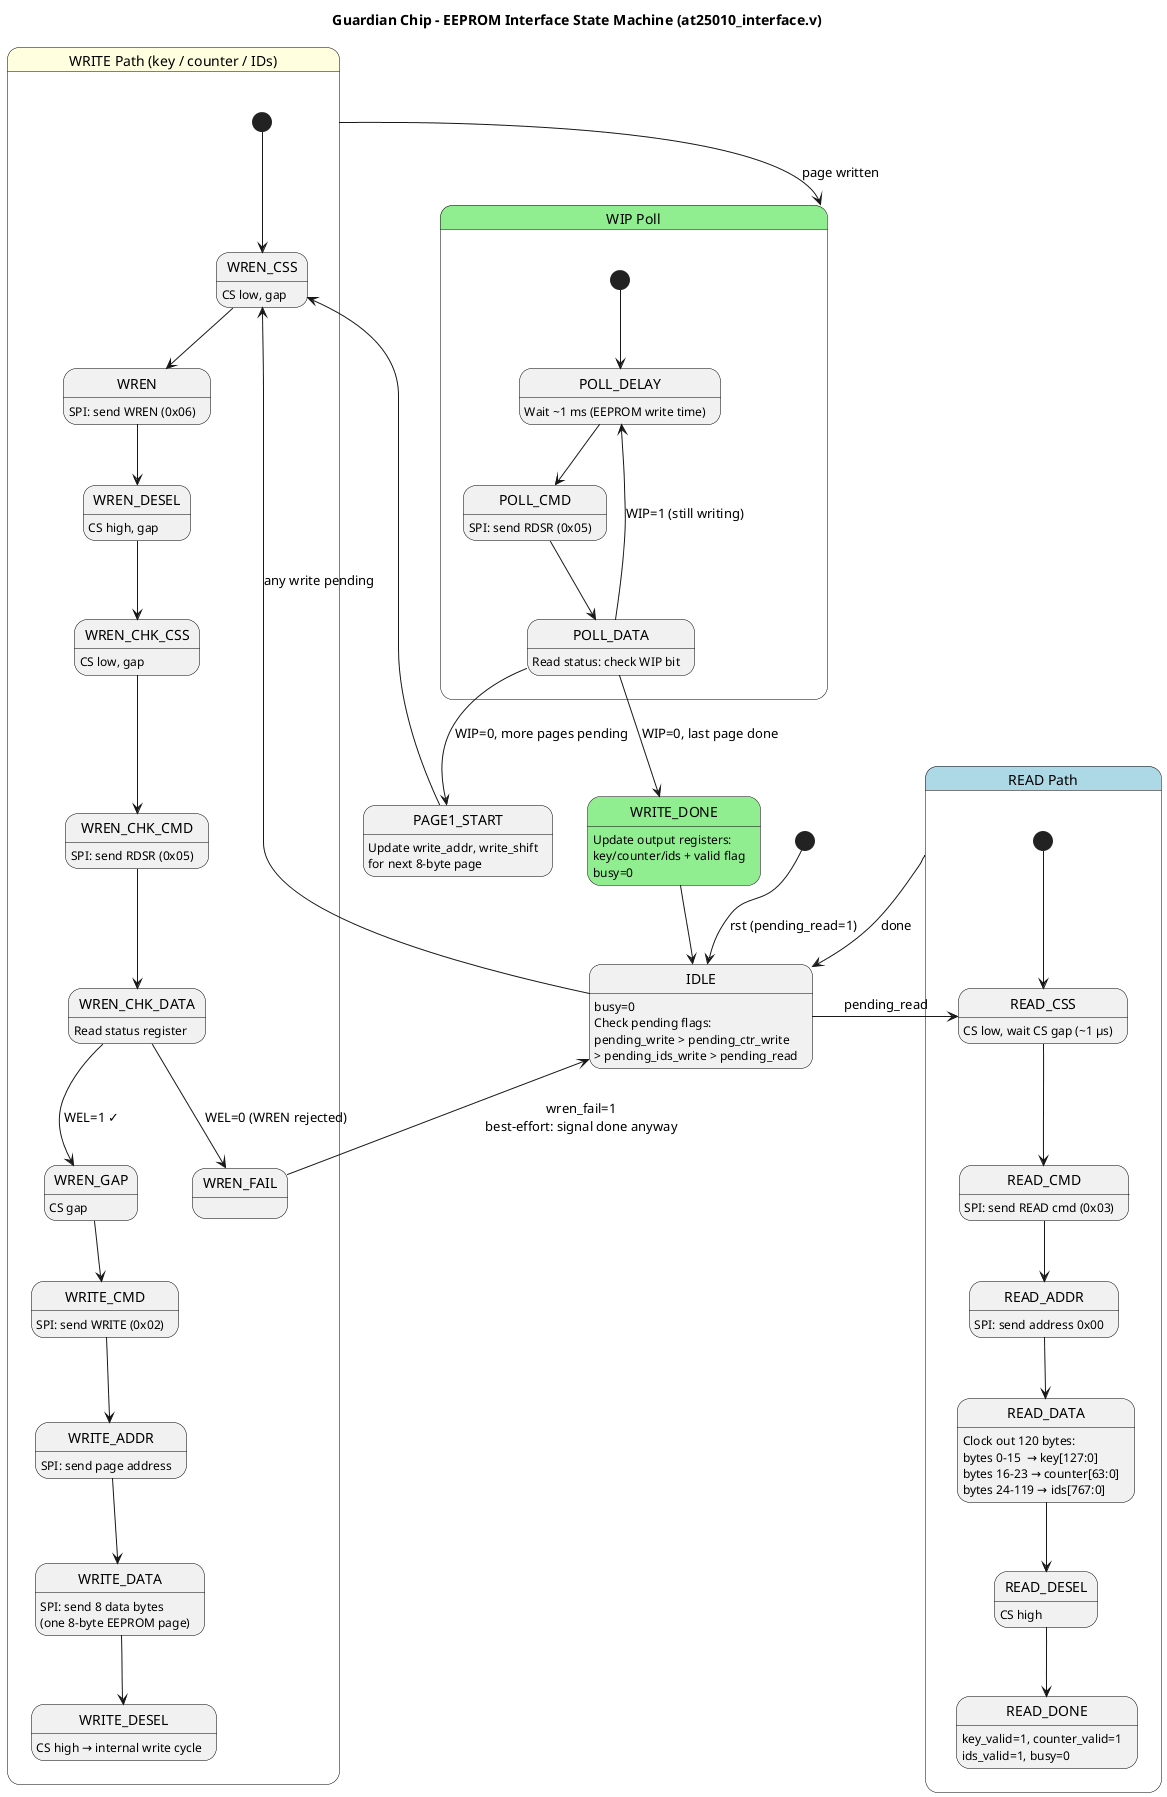
\includegraphics[height=0.82\textheight, keepaspectratio]{figures/eeprom_state.png}
  \caption{State machine of the EEPROM interface
           (\texttt{at25010\_interface.v}).
           A startup read is triggered automatically on reset.
           Write paths share the WREN/WEL verification and WIP polling logic.}
  \label{fig:eeprom_state}
\end{figure}

\subsection{LAYR Authentication Core (\texttt{layr\_core.v})}
\label{sec:impl:layr}

The LAYR core implements the complete protocol state machine described
in Section~\ref{sec:security:protocol}.
\Cref{fig:layr_state} shows all 29 states grouped by function.

\begin{figure}[p]
  \centering
  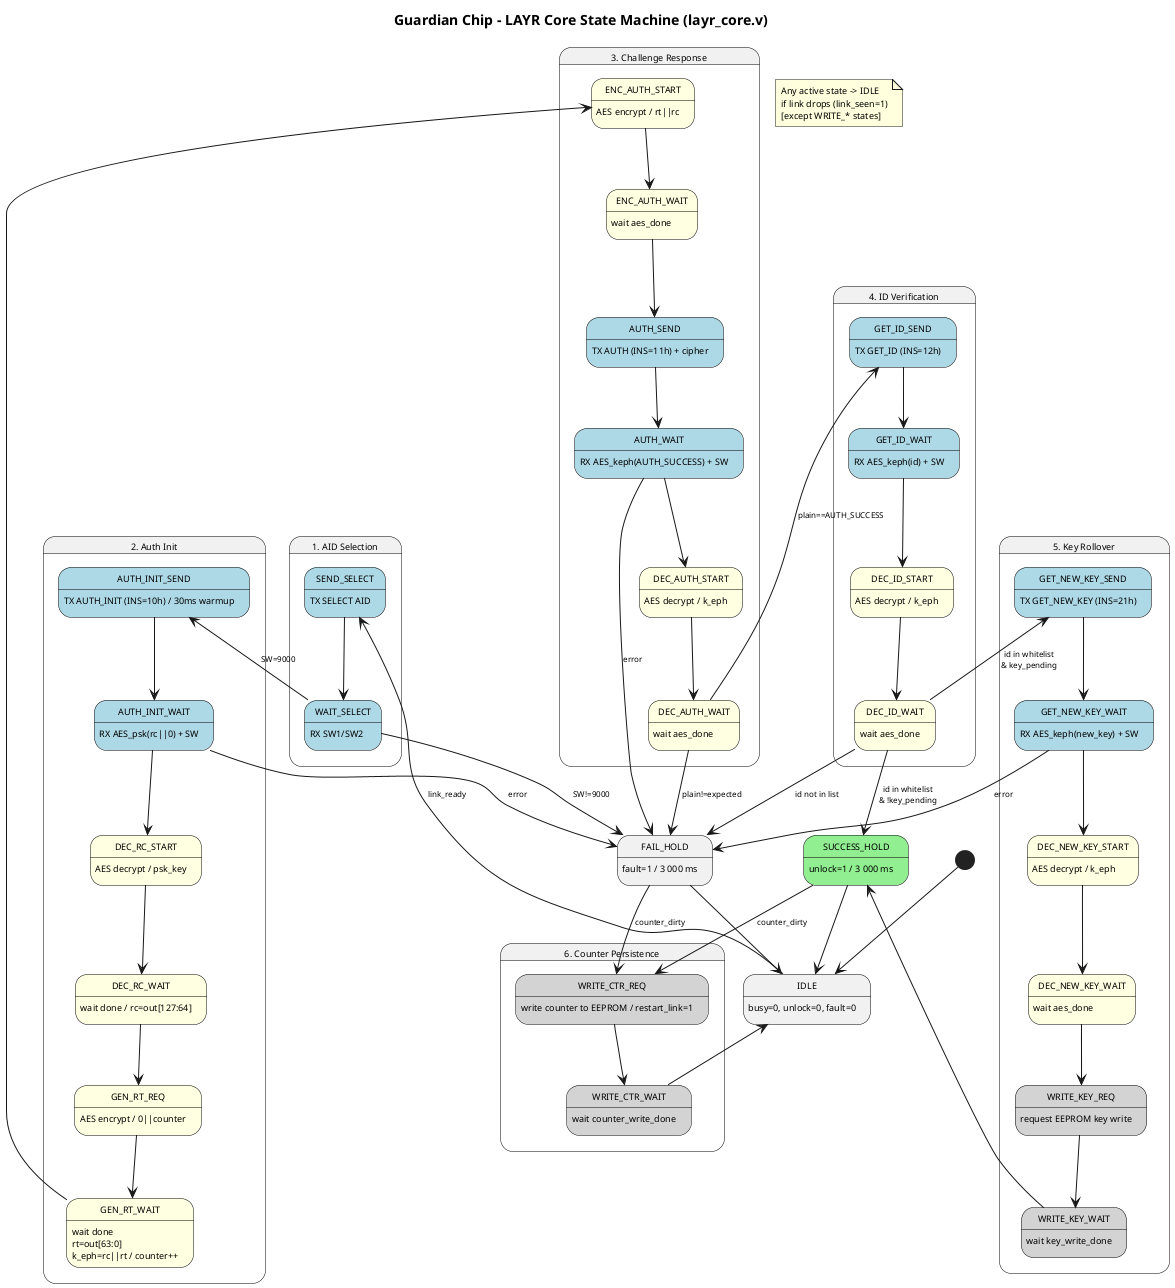
\includegraphics[width=0.92\textwidth, keepaspectratio]{figures/layr_auth_state.png}
  \caption{State machine of the LAYR authentication core
           (\texttt{layr\_core.v}).
           Yellow states invoke the AES engine;
           blue states exchange APDU bytes with the NFC interface;
           green states drive the unlock output.
           Any non-terminal state returns to IDLE if the NFC link drops.}
  \label{fig:layr_state}
\end{figure}

\paragraph{Status outputs.}
Three status output signals are driven from the LAYR core and
the EEPROM interface:
\begin{itemize}
  \item \texttt{status\_busy}: asserted whenever the LAYR core or
        EEPROM interface is active.
  \item \texttt{status\_unlock}: asserted for 3\,000\,ms after a
        successful authentication (and ID whitelist check).
  \item \texttt{status\_fault}: asserted for 3\,000\,ms on any
        authentication failure (wrong key, ID not in whitelist,
        protocol error, or NFC link fault).
\end{itemize}

\paragraph{Counter persistence.}
After every authentication attempt (success or failure) the
incremented nonce counter is written back to the EEPROM.
This operation is deliberately deferred until after the
HOLD state to minimise the latency perceived by the user at the door.
The LAYR core tracks whether the counter has been modified
(\texttt{counter\_dirty}) and triggers the write-back
via \texttt{counter\_write\_req} before returning to IDLE.

\paragraph{ID whitelist.}
The 96-byte whitelist region accommodates up to six 128-bit card
identities (ID~0 through ID~5).
A slot is considered empty if all 128 bits are zero.
During development, six default identities were pre-programmed into
the EEPROM for testing purposes.

\paragraph{Link recovery.}
If the NFC link drops unexpectedly (the card is removed mid-transaction),
the LAYR core detects the falling edge of \texttt{link\_ready}
and immediately returns to IDLE—provided it is not in a critical
section that must not be interrupted (such as an EEPROM write).
This prevents the machine from blocking indefinitely on missing APDU
responses.

% ===============================================================
\section{Android Simulator Application}
\label{sec:simulator}
% ===============================================================

No physical JavaCard was available during the majority of development;
one was only obtained at the very end of the project.
To enable software-level testing throughout the development process,
a companion Android application was developed that emulates the card
side of the LAYR protocol using Android's Host Card Emulation (HCE)
framework~\cite{roland2012hce}.

The application registers the AID \texttt{F000000CDC01} with the
Android NFC subsystem and implements the complete LAYR Level~1 card
protocol in a \texttt{HostApduService} (\texttt{CardService.kt}).
\Cref{tab:apdu_impl} summarises the implemented APDU commands.

\begin{table}[ht]
  \caption{APDU commands implemented by the Android simulator
           (class \texttt{CardService}).}
  \label{tab:apdu_impl}
  \centering
  \begin{tabular}{lllp{5cm}}
    \toprule
    Command & CLA & INS & Card behaviour \\
    \midrule
    SELECT AID   & 0x00 & 0xA4 & Reset state; return 0x9000 \\
    AUTH\_INIT   & 0x80 & 0x10 & Generate random $r_C$; return
                                  $\text{AES}_{k_\text{psk}}(r_C \| 0^{64})$ \\
    AUTH         & 0x80 & 0x11 & Verify $r_C$; compute $k_\text{eph}$;
                                  return $\text{AES}_{k_\text{eph}}(\texttt{AUTH\_SUCCESS})$ \\
    GET\_ID      & 0x80 & 0x12 & Return $\text{AES}_{k_\text{eph}}(\mathit{id})$;
                                  SW=0x9001 if new key pending \\
    GET\_NEW\_KEY& 0x80 & 0x21 & Return $\text{AES}_{k_\text{eph}}(k_\text{new})$ \\
    \bottomrule
  \end{tabular}
\end{table}

The user interface consists of three fragments (\cref{fig:app}):
\begin{itemize}
  \item \emph{Key}: the main fragment for regular Level~1
        authentication; displays the current transaction status
        (idle, communicating, success, failure) and the active PSK.
  \item \emph{Rollover}: configures the new key to be distributed
        in the next successful transaction and enables rollover mode,
        causing GET\_ID to return \texttt{SW=0x9001} so the terminal
        requests and stores the new key.
  \item \emph{Key Management}: allows updating the card's PSK by
        entering a 32-character hexadecimal string.
\end{itemize}

\begin{figure}[H]
  \centering
  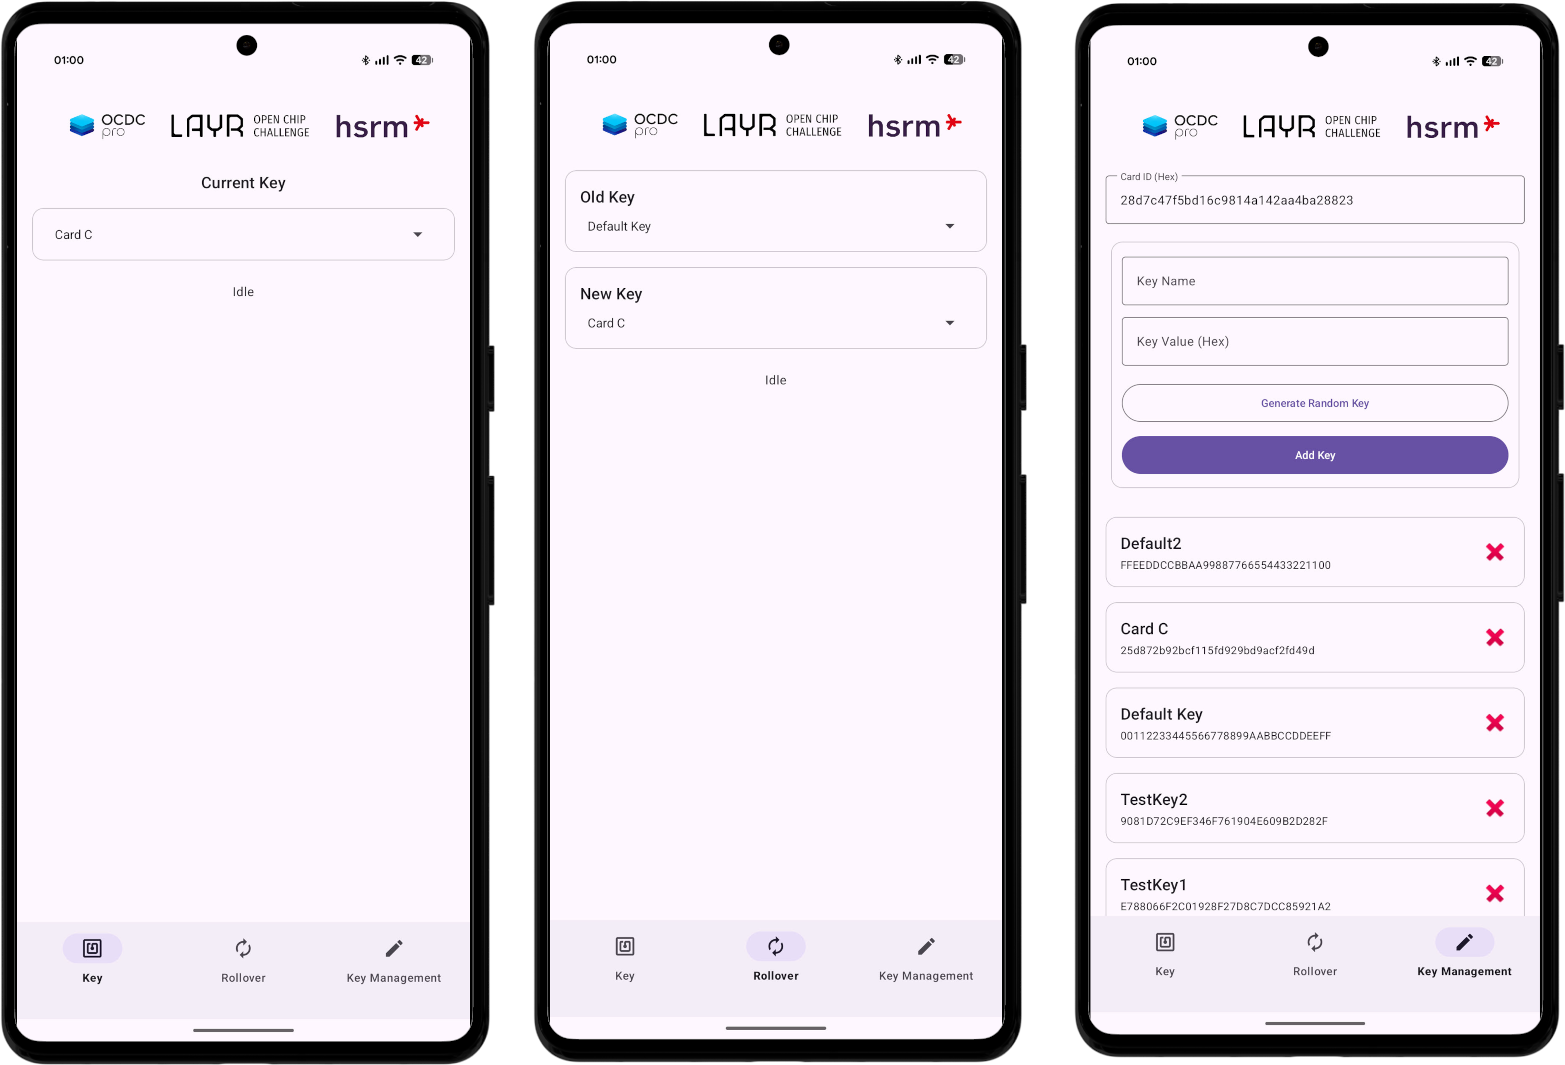
\includegraphics[width=0.6\linewidth]{figures/app.png}
  \caption{Android LAYR Simulator application showing the three
           fragments: Key (authentication status and active PSK),
           Rollover (key distribution) and Key Management (PSK update).}
  \label{fig:app}
\end{figure}

The application is intentionally kept simple—all cryptographic
operations use the standard Android \texttt{javax.crypto} AES/ECB
cipher—to match the hardware behaviour exactly and serve as a
ground truth for debugging.

\paragraph{Simulator limitation: JavaCard compatibility.}

A third-party LAYR protocol implementation rejected the Android HCE application
entirely.
The likely cause is that the implementation targeted JavaCards exclusively and
relied on card-specific behaviour that Android HCE does not reproduce exactly~--
for example, differences in APDU framing, ATS parameters, or response timing.
The Guardian Chip design was verified against both a physical JavaCard and the
Android HCE simulator without modification.

% ===============================================================
\section{Physical Design}
\label{sec:physical}
% ===============================================================

\subsection{Technology}
\label{sec:physical:tech}

The chip targets the IHP~SG13G2 130\,nm BiCMOS open-source
process~\cite{ihpsg13g2}.
SG13G2 provides a 130\,nm CMOS baseline layer stack suitable for
digital logic and has been released with a fully open-source PDK
under the Apache~2.0 license.
The submitted GDS will be physically manufactured by IHP,
with fabrication expected in 2026~\cite{ihp_mpp}.

\subsection{Pad Ring}
\label{sec:physical:pads}

The \texttt{chip\_top.sv} module instantiates the following IHP
pad cell types:
\begin{itemize}
  \item \texttt{sg13g2\_IOPadIn} for \texttt{sys\_clk}, \texttt{rst},
        \texttt{uart\_clk} (unused), \texttt{uart\_rx} (unused),
        and \texttt{spi\_miso}.
  \item \texttt{sg13g2\_IOPadOut30mA} for \texttt{uart\_tx} (idle-high),
        \texttt{spi\_sclk}, \texttt{spi\_mosi}, \texttt{cs\_0},
        \texttt{cs\_1}, and the three status outputs.
  \item \texttt{sg13g2\_IOPadInOut30mA} for the five user-IO
        bidirectional pads (currently held as inputs).
  \item Power pads: two \texttt{IOPadVdd}/\texttt{IOPadVss} pairs
        and one \texttt{IOPadIOVdd}/\texttt{IOPadIOVss} pair.
\end{itemize}

\subsection{Test Setup}
\label{sec:physical:testsetup}

All hardware tests were performed
on an ECP5-based ULX3S FPGA board as an interim development platform.
A custom 3D-printed case (FreeCAD source in \texttt{CAD/}) was
produced to mechanically integrate the ULX3S board, the MFRC522
reader, the EEPROM breakout, the relay and
the status LEDs into a demonstration unit (Figure~\ref{fig:testkit}).

\begin{figure}[H]
  \centering
  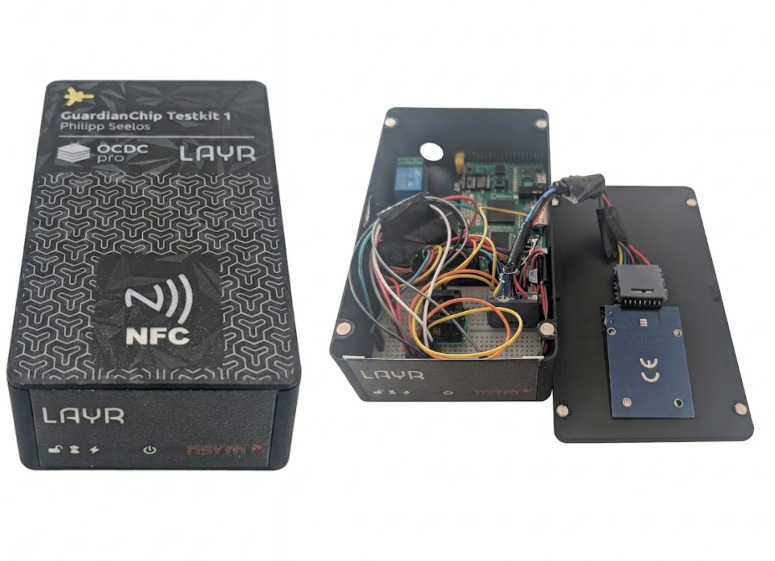
\includegraphics[width=0.75\linewidth]{figures/testkit.jpg}
  \caption{3D-printed demonstration enclosure housing the ULX3S FPGA
           development board, MFRC522 NFC reader, AT25010B EEPROM,
           relay, and status LEDs.
           CAD files (FreeCAD + STL) are located in \texttt{CAD/}.}
  \label{fig:testkit}
\end{figure}

% ===============================================================
\section{Development Process}
\label{sec:process}
% ===============================================================

This section describes the development timeline, the main challenges
encountered, and how they were resolved.
The project was carried out by a single person after the originally
planned team members withdrew from the challenge early in the project.
While this reduced the available resources, it also gave full
architectural control over all design decisions from the start.
It should be noted that the author had no prior experience with
ASIC design, Verilog/SystemVerilog, or SPI peripherals at the start
of the project. The learning curve across all three domains
simultaneously was steep and accounts for several of the detours
and delays described in this section.

\subsection{Phase 0: Simulation-First Approach and Its Limits}
\label{sec:process:phase0}

The project began in November~2025 with the intention to follow a
simulation-driven development methodology.
A set of testbenches was written using the Icarus~Verilog simulator
and the cocotb framework.
The idea was to verify each hardware interface module in simulation
before touching real hardware.

In practice, this approach did not work for the hardware interface
modules.
Correctly modelling the timing behaviour of the MFRC522 NFC reader
and the AT25010B EEPROM in a software simulation requires detailed,
cycle-accurate behavioural models of those devices—models that either
do not exist as open-source resources or would require more effort to
build than the hardware itself.
As a consequence, \emph{none} of the simulation-based testbench code
from this phase made it into the final design.
The lesson drawn was that for hardware interface modules,
simulation is a useful supplement but cannot replace testing on the
actual target hardware.

\subsection{Phase 1: Infrastructure and Basic SPI Communication}
\label{sec:process:phase1}

Because no official LAYR hardware kit was received, all external
components (MFRC522 reader, AT25010B EEPROM breakout, relay,
door lock and LEDs) had to be
procured and assembled independently.
A custom 3D-printed enclosure was designed in FreeCAD
and printed to integrate all components into a single demonstration
unit (see Section~\ref{sec:physical:testsetup} and \cref{fig:testkit}).

The initial development platform was an ECP5-based ULX3S FPGA board.
By late January~2026, basic SPI communication with the MFRC522
was established, and the chip was successfully reading the MFRC522
firmware version register as a first integration test.
Basic ISO~14443-A card detection with the anticollision sequence
was working shortly after.

\paragraph{First milestone: LAYR Level~0.}
With card detection working, a minimal access-control loop was
implemented that read the card's ISO~14443-A UID directly from
the MFRC522 and compared it against a hard-coded identifier.
Strictly speaking, LAYR Level~0 requires APDU-based communication
over ISO~14443-4; the UID check implemented here does not satisfy
this requirement, as the UID is obtained during the anticollision
procedure without establishing a transport layer.
This nonetheless constituted a first functional access-control
demonstrator by the end of January~2026 and confirmed that the
reader hardware and SPI driver were fundamentally sound.
Implementing full APDU-based mutual authentication—the LAYR
Level~1 requirement—proved to be a far harder problem, as the
following phase describes.

\paragraph{Debugging without instruments.}
During this phase the only available debugging tools were the
eight general-purpose LEDs on the ULX3S FPGA board (in addition
to the three dedicated status LEDs for unlock, busy, and fault).
Protocol state was encoded into bit patterns on these LEDs to indicate
which state the NFC detector state machine had reached.
This method proved sufficient for coarse-grained progress tracking
but made it nearly impossible to diagnose timing issues or inspect
individual SPI bytes.

\subsection{Phase 2: The APDU Dead-End and the Bootstrapping Problem}
\label{sec:process:phase2}

The central challenge of the project was implementing the ISO~14443-4
transport layer (APDU exchange) over the MFRC522.
This required two pieces of software to work correctly at the same time:
the MFRC522 driver on the FPGA, and the Android HCE application on the
card side.

\paragraph{The bootstrapping problem.}
Both components were developed simultaneously without an independent
reference implementation to verify either one against.
The MFRC522 driver could not be tested without a working card
emulator, and the Android HCE application could not be tested without
a working NFC terminal.
This mutual dependency created a bootstrapping problem:
any failure was ambiguous because the error could be in either component.

The Android application was written under the assumption that it
was correct, and the MFRC522 driver was then developed against that
assumption.
This led to an extended series of failed iterations
without clear diagnostic information—the FPGA would signal a fault
LED and provide no further detail.

\paragraph{Attempted detour: Verilog PN532 interface.}
With the Android HCE application producing no observable output and no
independent reference available, a different approach was explored:
replacing the MFRC522 with a PN532 NFC controller.
The PN532 implements the ISO~14443-4 transport layer in firmware,
exposing a higher-level host interface (HSU/SPI/I\textsuperscript{2}C)
that abstracts away raw frame handling.
The hope was that this would significantly reduce the protocol
complexity on the FPGA side—the host would only need to issue
high-level commands and receive complete APDUs, rather than managing
frame-level details manually.

A dedicated Verilog interface module for the PN532 was written and
initially brought up.
However, this approach was ultimately abandoned: integrating yet
another unproven component into an already failing system risked
compounding the ambiguity, and the time investment of adapting
the surrounding RTL was difficult to justify while the root cause of
the original failures remained unknown.

\paragraph{Resolution: PN532 as reference reader.}
The deadlock was eventually broken by using the PN532 in a different
role: not as a replacement for the MFRC522 in the FPGA design, but as
an independent reference terminal.
An Arduino sketch using the publicly available Seeed~PN532 library
(\texttt{seeed\_pn532})~\cite{seeed_pn532} was written to send APDU commands to the
Android phone via ISO~14443-4.
This provided, for the first time, an independent terminal that could
exercise the Android HCE application in isolation.

The test immediately revealed that the Android application had a
configuration error: the \texttt{HostApduService} was not correctly
registered in the Android manifest, so the operating system never
routed NFC APDUs to the application.
Once this was corrected, the PN532 sketch confirmed that the APDU
protocol logic in the application was functionally correct.

At approximately the same time, a logic analyser became available.
With both problems resolved—a confirmed working card emulator and
byte-level SPI visibility—the MFRC522 APDU driver was debugged and
brought to a working state within a short period.
The first end-to-end APDU exchange was achieved at the end of February~2026.

\paragraph{Lesson learned.}
The bootstrapping problem and the subsequent detour through a Verilog
PN532 interface together cost several weeks of development time.
In hindsight, procuring an independent reference NFC terminal at the
very start of the project—before any custom driver code was written—
would have allowed each component to be verified in isolation and
would likely have compressed this phase to a matter of days.
For future projects of this kind, establishing an independent
ground-truth implementation of every external interface before
beginning the primary development is strongly recommended.

\subsection{Phase 3: LAYR Protocol and System Integration}
\label{sec:process:phase3}

With a working ISO~14443-4 transport layer, the LAYR authentication
protocol was implemented in the \texttt{layr\_core} module.
A first version was tested with a hard-coded dummy key and confirmed
working in early March~2026.

The subsequent work focused on integration and area optimisation:
\begin{itemize}
  \item The AT25010B EEPROM interface was integrated so that the key,
        counter, and ID whitelist are loaded from non-volatile storage
        on power-up.
  \item A key-rollover mechanism was added on top of the standard
        LAYR~Level~1 protocol, allowing in-band key updates as part
        of an authenticated transaction.
  \item The single-cycle AES implementation was replaced by the custom
        iterative engine described in Section~\ref{sec:impl:aes},
        and the LFSR-based nonce generator was removed in favour of
        the AES-CTR construction.
  \item The \emph{coorus} composite-field S-box was integrated to
        further reduce the area of the AES core.
  \item An ID whitelist check with three pre-programmed default
        identities was added to the LAYR core.
\end{itemize}

\subsection{Phase 3b: JavaCard Compatibility and EEPROM Initialisation}
\label{sec:process:phase3b}

Once the Android HCE application worked reliably as a card emulator,
a physical JavaCard running the reference LAYR applet was obtained for
final validation.
Testing with the JavaCard exposed several timing and protocol issues
in the \texttt{mfrc522\_apdu\_interface} that had gone undetected with
the Android emulator, because Android's HCE framework is more tolerant
of non-conforming ISO~14443-4 behaviour than a hardware card.
Four specific fixes were applied to the module.
(1)~The I-block sequence number was not reset on card-detection restart,
causing the JavaCard to reject the first frame with a protocol error;
\texttt{block\_num} is now zeroed on every restart.
(2)~The ISO~14443-4 Start-up Frame Guard Time (SFGT) was not observed:
the JavaCard required a minimum 4.8\,ms gap after the ATS response,
while the Android emulator accepted frames immediately.
A 10\,ms SFGT wait state was inserted, and the MFRC522 timer registers
were reconfigured explicitly after the ATS exchange.
(3)~A card moved briefly out of range fires only \texttt{TimerIRq}
without an error bit; the original code treated this as a hard fault,
triggering a 3\,second lockout.
The fix performs a soft card-detection restart on timeout-only events.
(4)~The receive-length check required at least three bytes, rejecting
valid two-byte S(WTX) frames; the minimum was reduced to two bytes.

After these four fixes, the complete protocol ran successfully on both
the Android HCE emulator and the physical JavaCard.

\paragraph{EEPROM initialisation.}
To pre-programme the AT25010B EEPROM with the default key, nonce
counter, and card-identity whitelist, a dedicated FPGA bitstream was
built from the test module
\texttt{fpga/test/at25010\_write\_test\_top.v}.
This module burns a fixed set of parameters into the EEPROM at
power-up: the AES pre-shared key (\texttt{DEBUG\_KEY}),
an all-zero nonce counter, and six whitelist entries.
The first entry (\texttt{ID\_1}) is a fixed test identity
(\texttt{0x00\ldots01}).
The remaining five entries (\texttt{ID\_2} through \texttt{ID\_6})
contain the LAYR protocol identities of the cards and devices used
during hardware validation.
These identities are LAYR-layer values transmitted encrypted within
the APDU exchange and are distinct from the ISO~14443-A UIDs
exchanged during anticollision.
The bitstream was programmed once onto the ULX3S board with the
EEPROM connected; subsequent FPGA reconfigurations with the
production bitstream then load the pre-written values at startup.

\subsection{Phase 4: Tape-Out Preparation}
\label{sec:process:phase4}

Tape-out preparation involved adapting the RTL to the IHP~SG13G2 pad
cell library and iteratively resolving physical
verification failures that only manifest in the full back-end flow.
The two main challenges encountered—metal density fill and antenna
violations—are described in the following subsections.

\subsubsection{Metal Density Fill}
\label{sec:process:phase4:fill}

The IHP~SG13G2 PDK mandates a minimum metal fill density of~25\,\%
and a maximum of~75\,\% in every 800$\times$800\,\textmu{}m window
(rules \texttt{M2Fil.h}/\texttt{M3Fil.h} and \texttt{M2Fil.k}/\texttt{M3Fil.k})~\cite{ihpsg13g2}.
After place-and-route, the LibreLane KLayout filler step~\cite{librelane}
placed 1.0$\times$1.0\,\textmu{}m fill shapes on Metal~2 and Metal~3
with a default fill-to-fill spacing of 1.5\,\textmu{}m (M2) and 2.0\,\textmu{}m (M3).
Despite this, 13 local density violations remained on Metal~2 and Metal~3
in the high-density routing region (400--2000\,\textmu{}m from the core origin);
no violations occurred on any other metal layer.
The default KLayout filler is unable to correctly fill those tiles.
As an intermediate measure, reducing the fill-to-fill spacing in the PDK
filler macro (\texttt{sg13g2\_filler\_Metal.lym}) from 1.5\,\textmu{}m to
the DRC-minimum of 0.42\,\textmu{}m increased coverage and reduced the
violation count, but did not fully eliminate them.
Ultimately, these PDK-level changes proved unnecessary once the
\texttt{gdsfill}-based approach described below was adopted, and the
macro was left at its original default parameters.

To close the remaining violations, the open-source
\texttt{gdsfill}~\cite{gdsfill} tool was evaluated as a secondary fill pass.
\texttt{gdsfill} applies a combination of Track and Square tiling algorithms
on configurable 400\,\textmu{}m tiles to reach a user-specified target density,
using fill shapes of at least 1.0\,\textmu{}m width to satisfy the
\texttt{MFil.a1} minimum fill width rule.
Running it directly on the LibreLane output, however, introduced
over 200\,000 new \texttt{M2Fil.a2}/\texttt{M3Fil.a2} errors due to a
double-fill interaction: \texttt{gdsfill} placed shapes on top of
existing KLayout fill, and the DRC rule fires when merged shapes exceed
5\,\textmu{}m.

The fix consisted of three steps.
First, a dedicated KLayout script (\texttt{erase\_m2m3\_fill.py}) was
written to selectively erase the Metal~2 and Metal~3 filler layers
from the step-63 GDS before invoking \texttt{gdsfill}, leaving the
M1, M4, M5, TM1, and TM2 fill produced by the KLayout pass intact.
Second, the tile-boundary keep-out expansion in
\texttt{gdsfill}'s \texttt{prepare.py} was increased from the nominal
DRC spacing of 0.42\,\textmu{}m to 0.50\,\textmu{}m to account for
routing metal that straddles tile boundaries and is therefore invisible
to the fill-placement algorithm of the adjacent tile.
Third, the target fill density in \texttt{gdsfill\_config.yaml} was
raised from~35\,\% to~45\,\% so that tiles whose routing density already
exceeded~35\,\% would not be skipped, preventing \texttt{M2Fil.h}
violations that would arise if \texttt{gdsfill} left them unfilled.
The complete procedure was integrated into the build system as the
\texttt{gdsfill-clean-resume} Makefile target,
which backs up the filler GDS, erases M2/M3 fill, runs \texttt{gdsfill},
and then resumes the LibreLane flow from the density-check step onward.
To run the entire flow from scratch in a single step, the
\texttt{librelane-full-gdsfill-clean} target combines the full
synthesis and place-and-route run with the subsequent gdsfill pass.
Notably, no modifications to the PDK filler macro were required;
the default KLayout filler parameters remain unchanged and handle
all other metal layers correctly.
The resulting chip layout is shown in Figure~\ref{fig:klayout_final_gds}.

\begin{figure}[H]
  \centering
  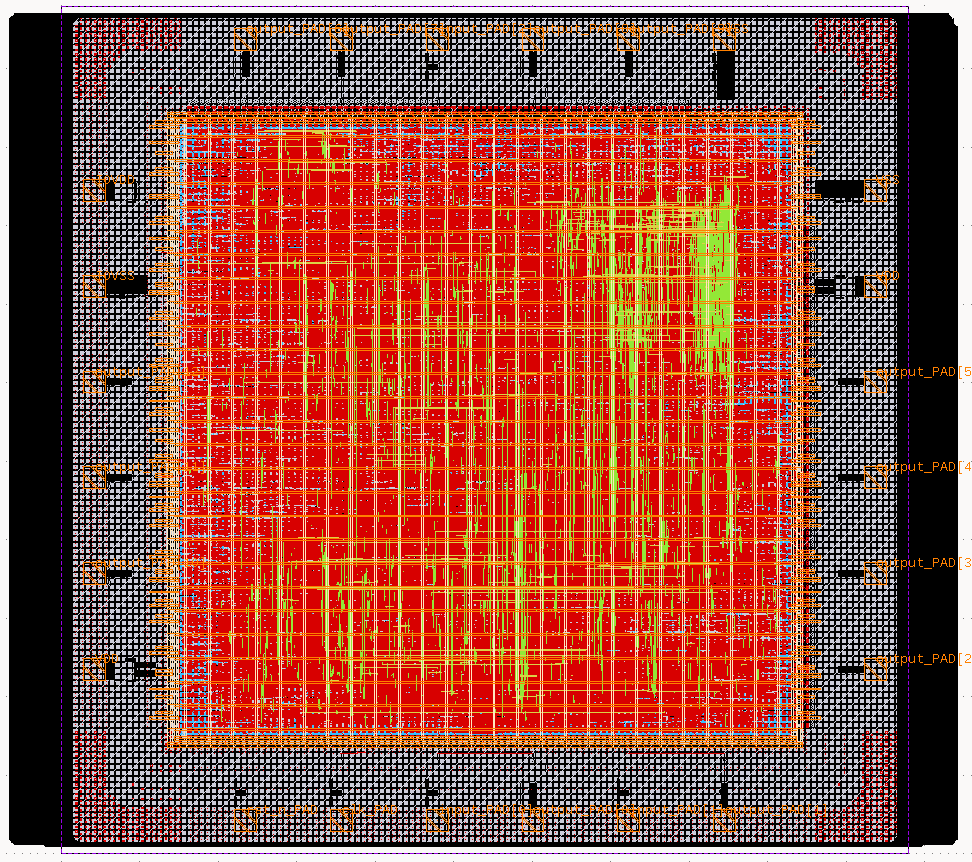
\includegraphics[width=0.33\columnwidth]{figures/klayout_final_gds.png}
  \caption{Final GDS of the Guardian Chip as viewed in KLayout after
           completion of the full LibreLane flow including metal density
           fill. The pad ring with 24 I/O pads is visible around the
           perimeter; the core logic occupies the central area.}
  \label{fig:klayout_final_gds}
\end{figure}

\subsubsection{Floating Nets and Antenna Violations}
\label{sec:process:phase4:antenna}

OpenROAD's post-routing antenna check reported 8~pin and 8~net
violations.
Inspection of the OpenROAD metrics revealed \texttt{timing\_\_drv\_\_floating\_\_nets:~4},
indicating that the router could not repair antenna effects on nets
without a fanout.
The root cause was in \texttt{chip\_core.sv}: the two unused input
pads \texttt{uart\_clk} and \texttt{uart\_rx} were connected only to
an AND-reduction expression assigned to a local signal
\texttt{\_unused}.
Yosys optimises such dead-end nets away during synthesis, leaving the
physical input pad nets without any downstream load.
The fix was to route each unused input directly to a corresponding
spare output pad---\texttt{uart\_clk} to \texttt{user\_io\_0} and
\texttt{uart\_rx} to \texttt{uart\_tx}---ensuring that the nets
connect two physical I/O cells and cannot be eliminated.
After this change, the KLayout antenna check reported zero violations
(\texttt{klayout\_\_antenna\_error\_\_count:~0}).

% ===============================================================
\section{Verification}
\label{sec:verification}
% ===============================================================

Functional verification was performed at two levels:
RTL simulation using the cocotb Python-based testbench framework,
and hardware validation on the ULX3S FPGA board with the Android
simulator application.

\paragraph{RTL simulation.}
The testbench directory (\texttt{cocotb/}) contains two Python-based
cocotb testbenches:
\begin{itemize}
  \item \texttt{test\_aes\_core.py} – unit tests for the AES engine
        using official NIST FIPS~197 vectors~\cite{fips197} plus
        round-trip encrypt/decrypt checks.
  \item \texttt{test\_layr\_core.py} – integration tests for the LAYR
        authentication core, covering successful authentication,
        rejected card (ID not in whitelist), wrong PSK, key rollover,
        and link-drop mid-transaction recovery.
        The testbench acts as both the NFC link and a software
        implementation of the card side using Python AES.
\end{itemize}

\paragraph{Hardware validation.}
The Android HCE application was used as a software card against the
FPGA prototype.
Because the application logs every received and transmitted APDU,
it was possible to verify the complete protocol flow byte-by-byte.
Test cases covered:
\begin{enumerate}
  \item Successful authentication with a whitelisted identity.
  \item Rejected card (identity not in whitelist).
  \item Wrong PSK key (AUTH step fails).
  \item Authentication followed by key rollover.
  \item Card removal mid-transaction (link-drop recovery).
\end{enumerate}

% ===============================================================
\section{Discussion}
\label{sec:discussion}
% ===============================================================

\paragraph{Security level.}
The current design fulfils LAYR Level~1 requirements.
Higher levels require additional hardware countermeasures against
physical attacks (e.g.\ power analysis or fault injection) that were
out of scope for this project.

\paragraph{Relay attacks.}
The LAYR Level~1 threat model explicitly includes active relay
attacks~\cite{hancke2005relay}, in which an adversary transparently
forwards NFC frames between a legitimate reader and a distant card.
The mutual challenge-response scheme prevents a \emph{replay} of a
previously recorded session, but does not inherently bound the
physical distance between card and reader during a live session.
A practical relay is constrained by the added round-trip latency
introduced by the relay channel; tightly timing the challenge-response
exchange at the application layer could provide a degree of distance
bounding.
This is not currently implemented and would be a meaningful extension
for deployments where the relay threat is significant.

\paragraph{Area and performance.}
The iterative AES design processes one round per clock cycle,
resulting in an 11-cycle latency at 32\,MHz (approximately 344\,ns).
A fully unrolled pipeline would reduce latency at the cost of area;
the current balance was chosen to fit within the QFN-24 area budget
and on the FPGA.
Post-layout metrics obtained from the completed LibreLane back-end run
are summarised in \cref{tab:area}.
The design comprises 49\,208 standard cells (of which 4\,833 are
sequential) plus 10\,275 timing-repair buffers inserted by OpenROAD.
The 2.699$\times$2.699\,mm die houses a 1.943$\times$1.943\,mm core
region at a standard-cell utilisation of 18.6\,\%, leaving substantial
routing headroom.
The chip is designed to operate at 32\,MHz, which is the clock
frequency assumed by all internal timing parameters (SPI baud rate,
millisecond timers, unlock duration).
The LibreLane synthesis constraint was deliberately set to 50\,MHz
to drive OpenROAD towards tighter timing closure and provide margin.
At the slow corner (1.08\,V, 125\,\textdegree{}C) setup timing is not
met at 50\,MHz; at 32\,MHz the available margin is approximately
13.7\,ns, which is sufficient for operation in that corner.
Estimated total power consumption at nominal conditions is 10.3\,mW.

\begin{table}[h]
  \centering
  \caption{Post-layout implementation summary (IHP SG13G2, LibreLane flow).}
  \label{tab:area}
  \begin{tabular}{lr}
    \toprule
    \textbf{Metric} & \textbf{Value} \\
    \midrule
    Die size                         & 2.699$\times$2.699\,mm (7.28\,mm$^2$) \\
    Core area                        & 1.943$\times$1.943\,mm (3.77\,mm$^2$) \\
    Standard-cell count              & 49\,208 \\
    \quad of which sequential        & 4\,833 \\
    Standard-cell utilisation        & 18.6\,\% \\
    Operating frequency              & 32\,MHz \\
    Synthesis timing target          & 50\,MHz (20\,ns period) \\
    Critical path (typ.\ corner)     & 17.5\,ns \\
    Setup slack @ 50\,MHz (typ.)     & $+$2.5\,ns \\
    Max.\ frequency (typ.\ corner)   & 57\,MHz \\
    Total wirelength                 & 4\,401\,mm \\
    Estimated power (nom.\ typ.)     & 10.3\,mW \\
    \bottomrule
  \end{tabular}
\end{table}

\paragraph{Nonce counter overflow.}
The 64-bit monotonic counter supports $2^{64}$ authentication
transactions before wrapping around.
Even if an adversary deliberately triggers failed authentication
attempts to force the counter forward, the enforced minimum
inter-transaction delay of 3\,seconds means that reaching a wrap-around
would take an astronomically long time, rendering this attack
entirely impractical.

% ===============================================================
\section{Conclusion}
\label{sec:conclusion}
% ===============================================================

This report presented the Guardian Chip, a compact NFC access-control
ASIC designed for the LAYR Open Chip Challenge~25/26.
The chip implements the LAYR Level~1 Authenticated Identification
Protocol over an ISO~14443-4 link, providing mutual AES-128
challenge-response authentication and session-key-protected ID transfer.

Key design choices include a shared SPI bus with EEPROM-first priority
scheduling, a single iterative AES-128 core using the \emph{coorus}
composite-field S-box (based on Canright's mathematics) for area
efficiency, a counter-based terminal nonce to avoid a dedicated random
number generator, and a key-rollover mechanism designed as an
additional feature on top of the LAYR~Level~1 specification
that binds key updates to successful authentication transactions.

A companion Android HCE application provides a fully software-based
card emulator for development and testing without requiring physical
JavaCards.
The design targets tape-out in the IHP~SG13G2 130\,nm process
using the LibreLane open-source ASIC flow.

% ---------------------------------------------------------------
% NFC state machine -- wide figure, placed here at the end
\begin{figure}[p]
  \centering
  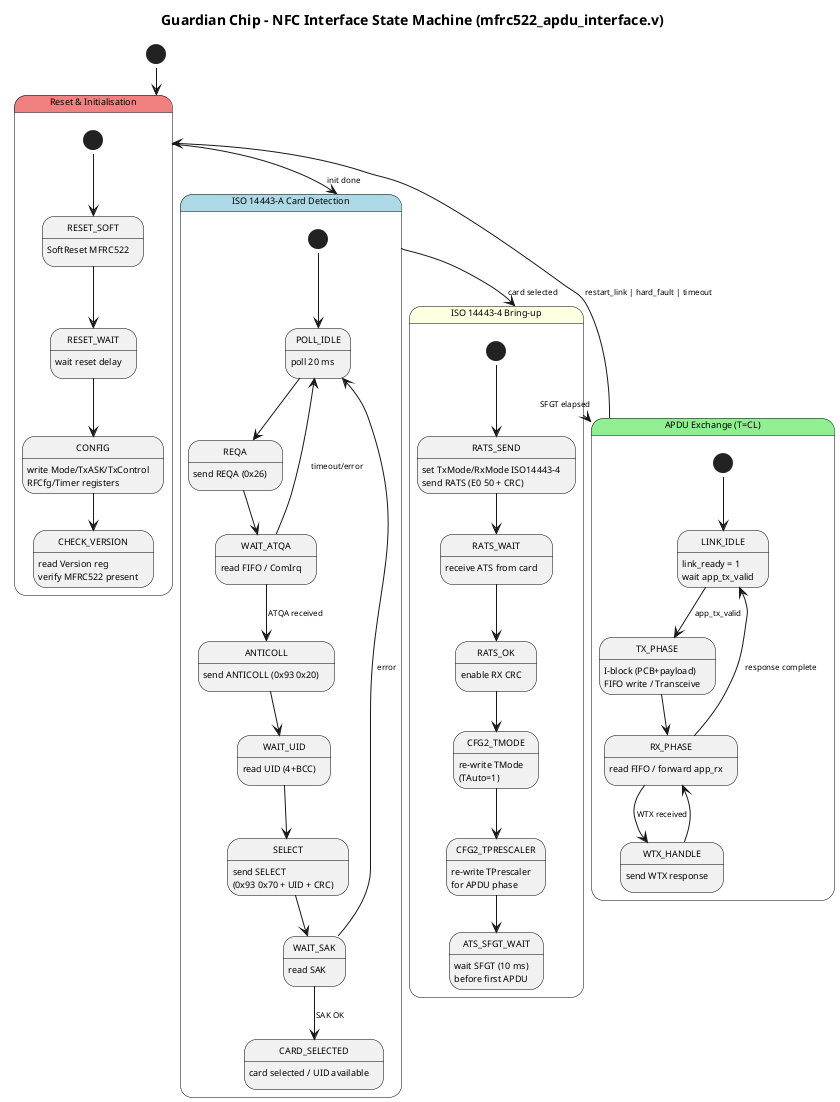
\includegraphics[height=0.8\textheight, keepaspectratio]{figures/nfc_link_state.png}
  \caption{State machine of the NFC interface module
           (\texttt{mfrc522\_apdu\_interface.v}).
           The four phase groups run left to right: hardware reset and
           configuration, ISO~14443-A card detection (REQA/ANTICOLL/SELECT),
           ISO~14443-4 link bring-up (RATS/ATS, timer reconfiguration,
           and SFGT wait), and transparent APDU I-block exchange
           including WTX handling.}
  \label{fig:nfc_state}
\end{figure}

% ---------------------------------------------------------------
\section*{Acknowledgements}
The author thanks Prof.\,Dr.\ Steffen Reith (Hochschule RheinMain)
for supervision and guidance throughout this project.

% ---------------------------------------------------------------
\section*{AI Usage Disclosure}
Parts of this work made use of large language model (LLM) assistance.
Specifically, an LLM was used to generate initial Verilog/SystemVerilog
code that served as a starting point for subsequent manual debugging,
bug fixes, and improvements; to generate initial Android application
code (HCE service, APDU handling) that similarly served as a basis for
manual refinement; to assist with interpreting SPI signal traces and
cross-referencing them against peripheral datasheets; and to draft and
refine portions of this report.
All generated code was reviewed, tested, and modified by the author.

% ---------------------------------------------------------------
\bibliographystyle{ACM-Reference-Format}
\bibliography{references}

\end{document}
